\documentclass[FM,BP]{tulthesis}

\newcommand{\verze}{2.1}

\usepackage{polyglossia}
\setdefaultlanguage{czech}


\usepackage{makeidx}
\makeindex

\usepackage{fontspec}
\usepackage{xunicode}

\usepackage{xltxtra}
\usepackage{tabularx}

\usepackage{tikz}
\usepackage{bbding}
\usepackage{graphicx}
\usepackage{float}
\usepackage{lscape}
\usepackage{nameref}
\usepackage[format=plain,
            labelfont=it,
            textfont=it]{caption}
\usepackage{amsmath}
\graphicspath{ {./images}{./tex-tul-template} }

% příkazy specifické pro tento dokument / specific commands for this document
\newcommand{\argument}[1]{{\ttfamily\color{\tulcolor}#1}}
\newcommand{\argumentindex}[1]{\argument{#1}\index{#1}}
\newcommand{\prostredi}[1]{\argumentindex{#1}}
\newcommand{\prikazneindex}[1]{\argument{\textbackslash #1}}
\newcommand{\prikaz}[1]{\prikazneindex{#1}\index{#1@\textbackslash #1}}
\newcommand{\ccheckmark}{{\color[HTML]{009901} \CheckmarkBold}}
\newcommand{\ccrossmark}{{\color[HTML]{CB0000} \XSolid}}
\newenvironment{myquote}{\begin{list}{}{\setlength\leftmargin\parindent}\item[]}{\end{list}}
\newenvironment{listing}{\begin{myquote}\color{\tulcolor}}{\end{myquote}}
\clubpenalty=10000
\widowpenalty=10000
\sloppy

% deklarace pro titulní stránku / title page declaration
\TULtitle{Řešení problematiky informačního systému střední školy}{}
\TULauthor{Daniel Adámek}

% pro bakalářské, diplomové a disertační práce / for bachelor, master theses and dissertation
\TULprogramme{B0613A140005}{Informační technologie}{Information technology}
\TULbranch{}{Aplikovaná informatika}{Applied Informatics}
%\TULbranch{1802T008}{Nějaký jiný obor}{Some other branch}
\TULsupervisor{Ing. Lenka Kosková Třísková Ph.D.}
\TULyear{2024}

% pro habilitační práce / habilitation thesis
%\TULbranch{}{Technická kybernetika}{Technical cybernetics}
%\TULyear{2022}

% Použití bibLateXu, pracuje s ISO stylem
% BibLaTeX settings, works with ISO style
\usepackage[ 
    backend=biber
    % ,style=iso-authoryear % styl vyžaduje FZS TUL , místo příkazu \cite{} je potřeba využít \parencite{} (sazba kulatých závorek) / style required by FZS TUL use \parencite{} instead of \cite{}
    ,style=iso-numeric
    ,style=numeric
    ,sortlocale=cs_CZ
    ,autolang=other
    ,bibencoding=UTF8
    %,urldate=edtf
    ,maxcitenames=2 %maximum v textu citovaných jmen
    ,maxbibnames=3 %maximum v seznamu vyjmenovaných autorů
    ]{biblatex}

\addbibresource{refs.bib}% vložení seznamu literárních zdrojů v bib formátu / input of references in bib format

% Úprava iso-numeric.bbx v souladu s požadavky TUL hranaté závorky v číslovaném seznamu / Modification of iso-numeric.bbx in accordance with TUL requirements of square brackets in a numbered list
\DeclareFieldFormat{labelnumberwidth}{\mkbibbrackets{#1}}

% Formátování podle pokynů FZS, při využití stylu iso-authoryear, čárka mezi jmény a poslední jméno se spojkou a / special requirements of FZS TUL 
\DeclareDelimFormat{multinamedelim}{\addcomma\space}

\DeclareDelimFormat{finalnamedelim}{%
  \ifnumgreater{\value{liststop}}{2}{\finalandcomma}{}%
  \addspace\bibstring{and}\space}

\DeclareNameAlias{author}{family-given/given-family} 
%%%%%%%%%%%%%%%%%%%%%%%%%%

\usepackage{csquotes} %užití biblatexu hlasí warnings, důvodem může být použití českých uvozovek v citacích! / solving of problems with Czech quotations
\urlstyle{same} %sazba url odkazů stejným fontem jako ostatní text, řešení problémů v zalamování hypertextových odkazů v citacích / url in references setting into the same form as text 


\begin{document}

% Prohlášení
\ThesisStart{male}
%\ThesisStart{zadani-a-prohlaseni.pdf}

% Abstrakt
\begin{abstractCZ}
    Tato bakalářská práce se primárně zaměřuje na návrh a implementaci nových komponent pro řešení stávajícího informačního systému střední průmyslové školy, s cílem eliminovat identifikované slabiny a využít potenciál pro zlepšení. Práce vychází z podrobné analýzy současného stavu systému, včetně jeho funkcionalit, toku dat, synchronizačních procesů, API rozhraní, legislativních požadavků a bezpečnostních opatření. Na základě zjištěných výsledků se práce soustředí na návrh a implementaci klíčových funkcí pro efektivnější správu školy a odbourání automatizovatelných a repetetivních úkonů. Důraz je kladen na praktickou aplikovatelnost navrhovaných řešení, jejich integraci do stávajícího systému a možnost dalšího rozvoje.
\end{abstractCZ}

\begin{keywordsCZ}
    informační systém, návrh, in-house vývoj, školství
\end{keywordsCZ}
    
    \vspace{2cm}
    
\begin{abstractEN}
    This bachelor thesis primarily focuses on the design and implementation of new components for the solution of the existing information system of a secondary industrial school, with the aim of eliminating identified weaknesses and exploiting the potential for improvement. The work is based on a detailed analysis of the current state of the system, including its functionalities, data flow, synchronization processes, API interfaces, legislative requirements and security measures. Based on the findings, the thesis focuses on the design and implementation of key features for more efficient school management and the elimination of automated and repetitive tasks. Emphasis is placed on the practical applicability of the proposed solutions, their integration into the existing system and the possibility of further development.
\end{abstractEN}
    
\begin{keywordsEN}
    information system, design, in-house development, education
\end{keywordsEN}

% Volná stránka
\clearpage

% Poděkování
\begin{acknowledgement}
    Prvně bych rád vyjádřil svou vděčnost Střední průmyslové škole elektrotechnické, Praha 2, Ječná 30, kterou zastupuje ředitel Ing. Bc. et Bc. Ondřej Mandík ING-PAED IGIP. Bez jeho laskavosti a podpory by toto dílo nebylo možné realizovat. Škola mi poskytla nezbytné informace, umožnila mi upravit svůj informační systém.. Tato zkušenost byla pro mě nesmírně cenná a pomohla mi v mnoha studijních i pedagogických aspektech.
    
    Zvláštní poděkování patří všem zaměstnancům školy a mým kolegům pedagogům, kteří mi pomohli kritickým pohledem na stávající systém a při hledání nových, lepších řešení. Jejich nápady a zpětná vazba byly jedním z klíčových aspektů pro vytvoření nového informačního systému, který je efektivní.
    
    Dále bych chtěl poděkovat všem členům mého vedení, rodině a přátelům, kteří mi poskytli cennou pomoc a podporu během procesu vytváření této bakalářské práce. Jejich trpělivost, porozumění a povzbuzování bylo pro mě během celého procesu klíčové.
    
    Nakonec bych chtěl vyjádřit svou vděčnost všem, kteří se na tomto díle podíleli, ať už přímo nebo nepřímo. Bez jejich kolektivního úsilí a podpory by tento projekt nebyl možný. Vaše práce a podpora byla cenná a jsem vám za to hluboce vděčný.
    
    Děkuji všem.
\end{acknowledgement}

% Obsah
\phantomsection\addcontentsline{toc}{section}{Obsah}
\tableofcontents
\clearpage

% Seznam zkratek
\begin{abbrList}
    \textbf{FM TUL} & Fakulta mechatroniky, informatiky a mezioborových studií
    Technické univerzity v~Liberci \\
    \textbf{SPŠE Ječná} & Střední průmyslová škola elektrotechnická, Praha 2, Ječná 30 \\
    \textbf{MŠMT} & Ministerstvo školství, mládeže a tělovýchovy \\
    \textbf{IS} & Informační systém \\
    \textbf{ŠIS} & Školní informační systém \\
    \textbf{OVM} & Orgán veřejné moci \\
    \textbf{NSESSS} & Národní standard pro elektronické systémy spisové služby \\
    \textbf{UCD} & User Centered Design
\end{abbrList}

% ====================================================================== %

% Udržitelnost
\chapter{Udržitelnost}
Udržitelnost informačního systému (IS) je klíčová pro jeho dlouhodobé úspěšné fungování a adaptaci na měnící se potřeby školy. Udržitelný IS musí být navržen tak, aby byl flexibilní, modulární a schopný integrace nových technologií a procesů. Toto zajišťuje, že systém zůstane relevantní, efektivní a schopen růstu spolu s organizací, aniž by bylo nutné jej zásadně předělávat nebo nahrazovat.

Při návrhu nových komponent IS je nezbytné přistupovat s předvídavostí a zaměřením na rozšiřitelnost. Nové komponenty by měly být navrženy tak, aby bylo možné je v budoucnu jednoduše upravovat, rozšiřovat o nové funkce nebo integrovat s dalšími systémy a technologiemi.

Základem udržitelnosti a rozšiřitelnosti IS je také kladen důraz na kvalitu kódu, dokumentaci a testování. Kvalitní, dobře dokumentovaný a otestovaný kód usnadní úpravy a rozšiřování systému. To do budoucna pomůže předcházet chybám, které by mohly vzniknout při integraci nových komponent nebo při rozšiřování funkcionalit.

% Spisová služba
\chapter{Správa agendy tříd a žákovských skupin}

Ve vzdělávacích systémech je běžnou praxí rozdělovat studenty do tříd a následně do menších skupin pro různé předměty a aktivity, neboť tento postup významně přispívá k efektivitě vzdělávacího procesu jak pro žáky, tak pro učitele. Dělba studentů do menších skupin umožňuje přizpůsobit výuku individuálním potřebám žáků, což zvyšuje jejich zapojení a porozumění látce. Příkladně v jazykových předmětech je nezbytné vést aktivní konzultace, které jsou v menších skupinách realizovatelné mnohem efektivněji. 

Dalším důvodem pro dělení žáků je kapacitní omezení učeben, které by při výuce v rámci celého třídního kolektivu nebylo možné optimálně využít. Tato opatření vedou k vyšší kvalitě výuky a efektivnějšímu využití dostupných zdrojů.

\subsection*{Definice}

\textbf{Class \( C \)}: třída je množina všech studentů a je označena jako \( C \). Formálně:

\[
C = \{ s_1, s_2, \ldots, s_n \}
\]

kde \( s_k \) je student a \( n \) je celkový počet studentů ve třídě.

\textbf{SubClass \( SC_{i/j} \)}: žákovská skupina (dále jen skupina) je podmnožina třídy \( C \), kde \( i \) je číslo skupiny a \( j \) je počet částí. Formálně:

\[
SC_{i/j} \subset C \quad
\]

\subsection*{Podmínky pro skupiny}

Abychom zajistili, že žádný student není opomenut a že všechny skupiny jsou disjunktní, musí být splněny následující podmínky:

\subsubsection*{Úplnost}

Sjednocení všech \( j \) částí skupiny musí tvořit celou třídu \( C \):

\[
\bigcup_{i=1}^{j} SC_{i/j} = C
\]

\subsubsection*{Disjunkce}

Žádný student nesmí patřit do více než jedné části téže skupiny:

\[
SC_{i/j} \cap SC_{k/j} = \emptyset \quad \text{pro} \quad i \neq k
\]

\subsection*{Kategorizace podmnožin}

V rámci tříd můžeme studenty rozdělit do různých kategorií podmnožin podle různých kritérií. Níže uvádíme několik obecných kategorií podmnožin a příklad jejich využití.

\subsubsection*{Dělení na zlomky}

Jedním z nejběžnějších způsobů rozdělení třídy je dělení na zlomky. Tato metoda je často využívána pro různé aktivity a předměty, kde je potřeba pracovat s menšími skupinami studentů.

\setlength{\parindent}{0em}
\setlength{\parskip}{1em}
\textbf{Příklad}: Rozdělení třídy na dvě poloviny:

\[
SC_{1/2} \quad \text{a} \quad SC_{2/2}
\]

kde:

\[
SC_{1/2} \cup SC_{2/2} = C
\]

a

\[
SC_{1/2} \cap SC_{2/2} = \emptyset
\]

Tento přístup je užitečný například při laboratorních cvičeních, kde je potřeba, aby každý student měl přístup k vybavení a učitel mohl efektivně dohlížet na práci studentů.

\subsubsection*{Dělení podle pohlaví}

Další běžnou metodou rozdělení studentů je podle pohlaví. Toto rozdělení může být užitečné v situacích, kde je potřeba řešit specifické potřeby studentů podle pohlaví.

\begin{samepage}
\setlength{\parindent}{0em}
\setlength{\parskip}{1em}

\textbf{Příklad}: Rozdělení třídy na dívky a chlapce:
\nopagebreak

\[
SC_{\text{dívky}} \quad \text{a} \quad SC_{\text{chlapci}}
\]
\nopagebreak

kde:
\nopagebreak

\[
SC_{\text{dívky}} \cup SC_{\text{chlapci}} = C
\]
\nopagebreak

a
\nopagebreak

\[
SC_{\text{dívky}} \cap SC_{\text{chlapci}} = \emptyset
\]

Tento přístup může být užitečný při tělesné výchově nebo v předmětech, kde jsou specifické fyziologické nebo psychologické rozdíly mezi pohlavími relevantní.
\end{samepage}

\subsection*{Důsledky a diskuse}

\subsubsection*{Úplnost}

Podmínka úplnosti zajišťuje, že každý student ve třídě \( C \) je přiřazen do alespoň jedné skupiny. Pokud by některý student nebyl zahrnut v žádné skupině, nebyla by splněna podmínka:

\[
\bigcup_{i=1}^{j} SC_{i/j} \neq C
\]

To by znamenalo, že existuje alespoň jeden student \( s_k \), který nepatří do žádné části skupiny, což je nepřijatelné.
\pagebreak
\begin{samepage}
\subsubsection*{Disjunkce}

Podmínka disjunkce zajišťuje, že žádný student není přiřazen do více než jedné části skupiny. Pokud by některý student patřil do více než jedné části skupiny, byla by narušena disjunkčnost:
\nopagebreak

\[
SC_{i/j} \cap SC_{k/j} \neq \emptyset \quad \text{pro} \quad i \neq k
\]
\nopagebreak

To by znamenalo, že existuje alespoň jeden student \( s_k \), který patří do více než jedné části skupiny, což je také nepřijatelné.
\end{samepage}

\subsection*{Příklady}

\subsubsection*{Třída a Skupiny}

Předpokládejme, že máme třídu \( C \) se \( n \) studenty:

\[
C = \{ s_1, s_2, \ldots, s_n \}
\]

Dále předpokládejme, že třídu \( C \) chceme rozdělit do \( j \) disjunktních skupin:

\[
\{ SC_{1/j}, SC_{2/j}, \ldots, SC_{j/j} \}
\]

\subsubsection*{Úplnost}

\[
\bigcup_{i=1}^{j} SC_{i/j} = C
\]

Tento výraz zajišťuje, že každá část skupiny je zahrnuta ve sjednocení, což pokrývá celou třídu.

\subsubsection*{Disjunkce}

\[
SC_{i/j} \cap SC_{k/j} = \emptyset \quad \text{pro} \quad i \neq k
\]
Tento výraz zajišťuje, že žádný student není zahrnut ve více než jedné části skupiny.

\begin{samepage}
\subsubsection*{Příklad pro tři části}

Pro ilustraci uvažujme třídu \( C \) se šesti studenty:
\nopagebreak
\[
C = \{ s_1, s_2, s_3, s_4, s_5, s_6 \}
\]

\noindent
Chceme třídu rozdělit do tří disjunktních skupin:

\nopagebreak

\[
\{ SC_{1/3}, SC_{2/3}, SC_{3/3} \}
\]

\noindent
Předpokládejme, že:

\nopagebreak

\[
SC_{1/3} = \{ s_1, s_2 \}
\]
\[
SC_{2/3} = \{ s_3, s_4 \}
\]
\[
SC_{3/3} = \{ s_5, s_6 \}
\]

\noindent
Poté platí:

\[
SC_{1/3} \cup SC_{2/3} \cup SC_{3/3} = \{ s_1, s_2, s_3, s_4, s_5, s_6 \} = C
\]

\noindent
a

\[
SC_{1/3} \cap SC_{2/3} = \emptyset
\]
\[
SC_{1/3} \cap SC_{3/3} = \emptyset
\]
\[
SC_{2/3} \cap SC_{3/3} = \emptyset
\]
\end{samepage}

\subsection*{Matematický závěr}

Matematická úvaha o třídách a skupinách zajišťuje, že rozdělení studentů do skupin je úplné a disjunktní. To znamená, že každý student je přiřazen do alespoň jedné skupiny a žádný student není přiřazen do více než jedné části skupiny. Tímto způsobem je zajištěno, že žádný student není opomenut a že všechny skupiny jsou disjunktní a kompletně pokrývají celou třídu.


\section{Implementace}
V předchozí kapitole jsme diskutovali matematickou úvahu o třídách a jejich skupinách (SubClasses), kde jsme stanovili tři klíčové podmínky: úplnost, disjunkci a podmnožinovou strukturu. V této kapitole se zaměříme na implementaci těchto matematických principů do třídního a databázového modelu. Zároveň se pokusíme najít nejefektivnější řešení, které zajistí plnou konzistenci dat v databázi.

\subsection*{Třídní Model}

Třídní model zahrnuje několik hlavních entit: \texttt{Class}, \texttt{SubClass}, \texttt{Student} a \texttt{StudentAssignment}. Model \texttt{Class} reprezentuje třídu jako celek, model \texttt{SubClass} reprezentuje skupiny v rámci třídy, model \texttt{Student} reprezentuje jednotlivé studenty a model \texttt{StudentAssignment} zaznamenává přiřazení studentů k třídám a skupinám.

\subsubsection*{Class}

\texttt{Class} obsahuje informace o třídě, jako jsou identifikátor třídy, označení třídy, prefix, datum platnosti od a do, místnost a třídní učitel. 

\subsubsection*{SubClass}

\texttt{SubClass} reprezentuje skupiny studentů v rámci třídy. Každá skupina má své vlastní identifikační číslo, název a odkaz na třídu, ke které patří. SubClass může existovat pouze v kontextu třídy, což znamená, že každá SubClass musí být vždy přiřazena konkrétní třídě.

\subsubsection*{Student}

\texttt{Student} obsahuje informace o jednotlivých studentech, jako jsou identifikační číslo, uživatelské jméno, jméno a příjmení.

\subsubsection*{StudentAssignment}

\texttt{StudentAssignment} zaznamenává přiřazení studentů k třídám a skupinám. Obsahuje odkazy na studenty, třídy a skupiny, ke kterým jsou přiřazeni. Klíčovým prvkem tohoto modelu je zajištění trvanlivosti přiřazení, tedy schopnost zaznamenávat změny přiřazení studentů v průběhu roku. 

V průběhu školního roku mohou nastat různé změny, které vyžadují aktualizaci přiřazení studentů. Tyto změny mohou zahrnovat mnoho faktorů a ty nejčastější z nich jsou vyjmenovány níže. Trvanlivost přiřazení umožňuje udržovat historický záznam o všech těchto změnách, což je nezbytné pro správu.

\textbf{Problémy a důvody pro trvanlivost:}

\begin{itemize}
    \item \textbf{Přechody mezi třídami}: Studenti mohou být během školního roku přeřazeni do jiné třídy z různých důvodů, jako jsou změny nálad v třídním kolektivu nebo přestup studenta mezi obory.
    \item \textbf{Změny ve složení skupin}: V závislosti na specifických potřebách výuky mohou být studenti přeřazeni mezi různými skupinami. Například při výuce jazyků může být potřeba změnit složení skupin kvůli homogenizaci, nebo naopak heterogenizaci skupiny, čimž v závislosti na potřebách jednotlivých žáků lze docílit zefektivnění výuky.
\end{itemize}

Model \texttt{StudentAssignment} musí být schopen zaznamenávat všechny tyto změny, aby bylo možné udržovat konzistentní a aktuální přehled o přiřazení studentů. Tento model tedy umožňuje sledování přiřazení studentů k třídám a skupinám v určitém časovém období a zajišťuje, že historické změny jsou správně zaznamenány.

\textbf{Schopnosti modelu:}

\begin{itemize}
    \item \textbf{Referenční integrita}: Každý záznam o přiřazení musí odkazovat na platné záznamy ve třídách a skupinách.
    \item \textbf{Flexibilita přiřazení}: Umožňuje přiřazení studenta buď přímo do třídy nebo do specifické skupiny.
    \item \textbf{Trvanlivost}: Udržuje historické záznamy o přiřazení, které umožňují sledovat změny v průběhu školního roku.
\end{itemize}

Tímto způsobem model \texttt{StudentAssignment} nejen zajišťuje aktuálnost a konzistenci dat, ale také poskytuje cenné historické informace, které mohou být využity pro analýzu a zlepšení vzdělávacího procesu.

\begin{figure}[H]
    \centering
    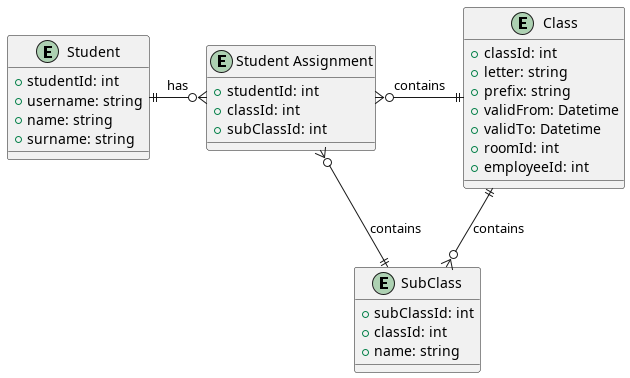
\includegraphics[width=\textwidth/2]{cd-student-assignment.png}
    \caption{Model tříd žákovských skupin}
    \label{fig:cd-student-assignment}
 \end{figure}

\subsection*{Databázový Model}

Databázový model musí zajistit, že všechny podmínky úplnosti, disjunkce a podmnožinové struktury jsou dodrženy. Toho lze dosáhnout pomocí správného nastavení cizích klíčů, unikátních omezení a triggerů.

\subsubsection*{Úplnost}

Úplnost zajišťuje, že každá třída je pokryta skupinami tak, aby žádný student nezůstal nezařazen. V aplikační logice zajistíme, že všechny skupiny dohromady pokrývají celou třídu. To můžeme kontrolovat při každém přiřazení studenta do skupiny. Je nezbytné, aby všechny skupiny třídy byly disjunktní a jejich sjednocení tvořilo celou třídu.

\subsubsection*{Disjunkce}

Disjunkci zajistíme na úrovni databáze pomocí unikátních omezení. Každý student může patřit pouze do jedné skupiny určitého typu v dané třídě. To lze implementovat pomocí unikátních indexů nebo pomocí aplikační logiky, která před přiřazením studenta do skupiny provede potřebné kontroly.

\subsubsection*{Podmnožinová struktura}

Podmnožinovou strukturu zajistíme pomocí cizích klíčů a referenční integrity. Každá skupina musí odkazovat na existující třídu a každé přiřazení studenta do skupiny musí odkazovat na existujícího studenta, třídu a skupinu.

\subsection*{Nejefektivnější řešení}

Pro zajištění úplné konzistence dat v databázi je nutné implementovat následující mechanismy.

\subsubsection*{Validace na úrovni aplikace}

Při každém přiřazení studenta do skupiny zkontrolujeme, zda přiřazení splňuje podmínky úplnosti a disjunkce. Pokud podmínky nejsou splněny, přiřazení se neprovede a uživatel obdrží příslušnou chybovou zprávu. Aplikační logika bude muset zohlednit také případy, kdy se celá třída učí společně a není třeba přiřazovat studenty do skupin.

\subsubsection*{Unikátní omezení}

Na úrovni databáze zavedeme unikátní omezení, která zajistí, že každý student může patřit pouze do jedné skupiny určitého typu v dané třídě. Tím zajistíme disjunkci dat.

\subsubsection*{Referenční integrita}

Pomocí cizích klíčů zajistíme, že každá skupina je podmnožinou existující třídy a každé přiřazení studenta odkazuje na existujícího studenta, třídu a skupinu. Tím zajistíme podmnožinovou strukturu.

\begin{figure}[H]
    \centering
    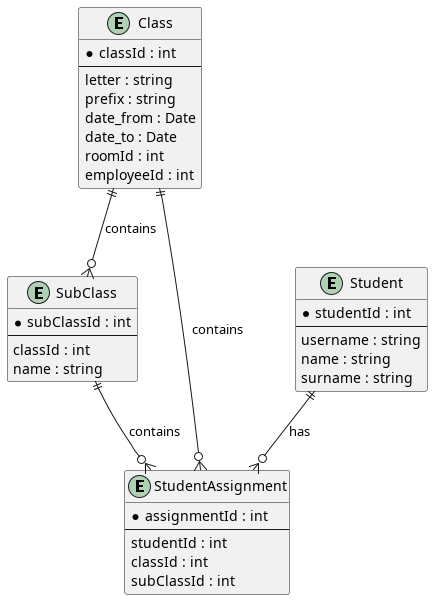
\includegraphics[width=\textwidth/2]{cd-referencni-identita.png}
    \caption{Referenční identita}
    \label{fig:cd-referencni-identita}
 \end{figure}

\subsection*{Diskuse o efektivitě řešení}

Implementace výše uvedených mechanismů v kombinaci s aplikační logikou poskytuje robustní řešení pro správu tříd a jejich skupin ve vzdělávacím systému. Validace na úrovni aplikace umožňuje flexibilitu a zajišťuje, že jsou splněny všechny matematické podmínky. Unikátní omezení a referenční integrita na úrovni databáze zajišťují konzistenci dat a minimalizují riziko chyb.

Tímto způsobem zajišťujeme:

\begin{itemize}
    \item \textbf{Úplnost}: Každá třída je kompletně pokryta skupinami a žádný student nezůstane nezařazen.
    \item \textbf{Disjunkce}: Každý student může být přiřazen pouze do jedné skupiny určitého typu v dané třídě.
    \item \textbf{Podmnožinová struktura}: Každá skupina je vždy podmnožinou konkrétní třídy, ke které patří.
\end{itemize}

% Notifikační systém
\chapter{Notifikační systém}
V rámci integrace spisové služby \ref{chap:integrace-spis-sluzby} do ŠIS se ukázalo jako nezbytné navrhnout dílčí komponentu - Notifikační systém. Tato komponenta představuje klíčový prvek pro efektivizaci procesů správy dokumentů a komunikaci v rámci školy. Jeho zavedení by mělo přispět k automatizaci generování a distribuce dokumentů, zrychlení procesů a snížení administrativní zátěže na personál.

Notifikační systém by měl být koncipován tak, aby poskytoval automatické notifikace o nových či změněných dokumentech, potřebě zpracování nebo schválení, a to všem relevantním stranám. Tím by se zvýšila transparentnost administrativních procesů a zefektivnila komunikace mezi třídními učiteli, administrativními pracovníky a vedením školy.

Při návrhu notifikačního systému je důležité přistupovat s ohledem na univerzálnost a rozšiřitelnost. Systém by neměl být omezen pouze na aktuální požadavky spojené s integrací spisové služby \ref{chap:integrace-spis-sluzby}, ale měl by být koncipován tak, aby snadno zvládal budoucí rozšíření a nová využití.

Tento přístup umožní využívat notifikační systém pro širokou škálu účelů, včetně informování žáků o nových známkách, upozornění učitelů na dlouhodobě nezapsanou absenci ve třídní knize, nebo dokonce automatické připomenutí důležitých školních událostí a termínů. Taková flexibilita znamená, že nofitikační systém se může stát důležitým prvkem komunikace podporujícím širokou škálu školních procesů a interakcí.

Navrhování systému s ohledem na budoucí potřeby a možnosti rozšíření je přístup, který zajišťuje, že investice vývoje přispěje k dlouhodobé udržitelnosti a přinese novou, trvalou hodnotu.

\section{Návrh řešení}
\begin{landscape}
    \begin{figure}[H]
        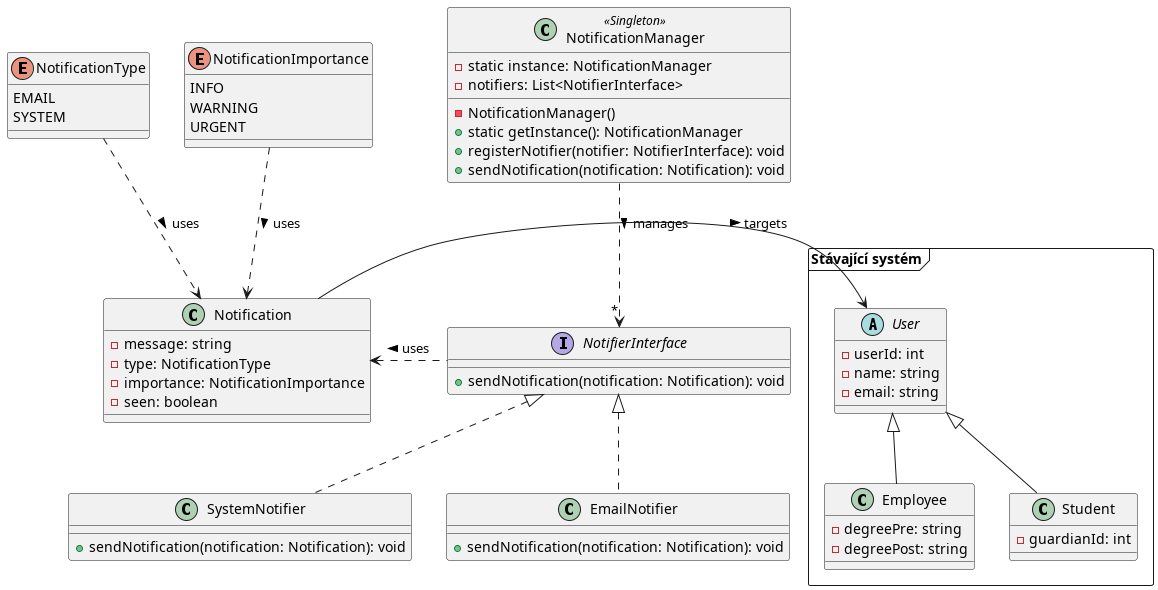
\includegraphics[width=\linewidth]{cl-notifikacni-system.png}
        \caption{Diagram tříd navrženého systému}
        \label{fig:cl-notifikacni-system}
    \end{figure}
\end{landscape}

\subsection*{Popis tříd, vztahů a návrhových vzorů}
Diagram \ref{fig:cl-notifikacni-system} zobrazuje architekturu notifikačního systému, který se skládá z několika komponent:
\begin{itemize}
    \item \textbf{NotifierInterface}: Toto rozhraní definuje základní metodu sendNotification(notification: Notification), která slouží k odesílání notifikací. Implementace tohoto rozhraní umožňuje vytvoření různých typů odesílatelů notifikací, jako jsou systémové notifikace nebo e-mailové notifikace.

    \item \textbf{Notification}: Třída reprezentuje samotnou notifikaci, obsahuje atributy jako message (text notifikace), type (typ notifikace, například EMAIL nebo SYSTEM), importance (důležitost notifikace, například INFO, WARNING, URGENT) a seen (boolean hodnota indikující, zda byla notifikace zobrazena).
    
    \item \textbf{NotificationType a NotificationImportance}: Enumerace, které definují možné typy a úrovně důležitosti notifikací. Pomocí těchto enumerací je možné jednoduše rozšířit systém o nové typy a priority notifikací.
    
    \item \textbf{User}: Abstraktní třída definující základní vlastnosti uživatelů systému, jako jsou userId, name a email. Tato třída je rozšířena třídami Employee a Student, které přidávají specifické atributy relevantní pro zaměstnance a studenty.
    
    \item \textbf{NotificationManager}: Třída, která využívá návrhový vzor Singleton, zajišťuje centralizovanou správu notifikací a jejich odesílatelů. Umožňuje registraci odesílatelů notifikací a zprostředkovává odesílání notifikací všem odesílatelům.
\end{itemize}
Návrh disponuje pouze několika atributy, které jsou, či budou reálně využívány.

Významným návrhovým vzorem použitým v tomto systému je Singleton, který je aplikován na NotificationManager k zajištění jediné instance správce notifikací v aplikaci. Tento vzor pomáhá udržovat konzistentní stav notifikací a zajišťuje, že všechny komponenty systému pracují s právě jedním objektem pro správu notifikací.


% ====================================================================== %

% Reference
\chapter{Reference}
\printbibliography[heading=none]

% Přílohy
\chapter{Přílohy}
\begin{itemize}
  \item Analýza pro proces modernizace školního informačního systému pro střední školu, Daniel Adámek
\end{itemize}

\end{document}
